\chapter{Search by Face Similarity}
\label{ch:face_search}

In this chapter, we propose another approach to the CBIR task. In this approach, we search only over the part of the dataset, which contains people. We ask if it is possible to find the target image based on the face of the person and faces of other people in the dataset.

This question arises from practical reasons. Once we investigated the V3C1 dataset, we realized that many of the images display people. We can use the previously investigated approach based on the location to find the target frame. However, with the increasing number of images showing people, it becomes difficult to retrieve the correct target image. Finding a similar face in an image search engine with the same background becomes difficult.

The technique described in this chapter works only on the feature space of faces. We first extract the faces from the dataset, and then we obtain a descriptor for each one of them. Based on the feature vectors, we organize the faces into a traversal structure supporting navigational commands.

The task of comparing the faces of the people and saying which look more similar has its roots in the human perception of the faces. Therefore, to evaluate the individual steps, we conduct experiments with real users.

Our experiments show that the feature space of the descriptors has limited power to order people based on the similarity in a way as people do. Despite that, we implement the traversal structure, which can be used with any new representation of the faces that could be developed in the future. Our last evaluations show that the median of the time required to find the target scene was smaller for our traversal approach than the baseline -- linear search.

\section{Task formulation}

\todo[inline]{}

\section{Extraction of the faces}

Face Detection is a widely studied problem. One of the key advancements in the past in this are was an article by \ref{} the authors speed up the human detection using Histogram of oriented gradients descriptor methods. Their method uses HOG description in combination with cascading classifiers. The method is quick and can perform even online. The disadvantage of the approach its lower performance on non-frontal views of the faces. Even today it is sometimes preferred due to its speed.

We followed more recent studies and decided to use a 

We followed the studies to come up to an CNN based approach for feature detection. The approach is described in the \cite{}. This was also implemented in Dlib library as an alternative to the HOG.



If we take a look at the dataset, we notice that only a small portion of the people present look directly into the camera. This comes from the fact, that these images are sampled from the videos, therefore, people are capture while doing some activity.

 algorithm to significantly speed up human detection using HOG descriptor methods. Their method uses HOG descriptors in combination with the cascading classifiers algorithm normally applied with great success to face detection


To extract the position of the faces from the dataset we used 

We used a smaller dataset for testing our hypothesis in this chapter. We work with only first 316 videos out of V3C1 dataset. We use the same extracted imgeas as in the previous chapter.


\todo[inline]{Dlib ako sme extrahovali}

\todo[inline]{dopisat slovy ze co vidime v datasete}
\todo[inline]{osekat zenu o aspon jednu riadok. napisat od 0.6 nevidime ziadnu podobnost}

We focused on the first 316 videos from V3C1 dataset to retrieve the faces available. The reason behind choosing 316 videos is purely to limit our experiments on the reasonably sized dataset, where the solution we will see later can be better tested. From these 316 videos, we were able to capture more than seventeen thousands faces. The distribution of the are covered by the faces is available in the figure \ref{}\todo{add figure}. Since most of the faces cover less than a 5\% of the screen, we decided to further clean the dataset.  To clean the dataset, we decided to go only with the faces, which covered at least ten percent of the picture. This resulted in obtaining 2047 faces. A random selection of faces is shown in the figure \ref{fig:random_selection_faces}. The This significantly reduces the size of the faces available
In the further sections we therefore work with 2047 faces from different people, in different angles. As in the example shown, we can also see one false positive. These were not manually checked, therefore we expect some.

\begin{figure}
    \centering
    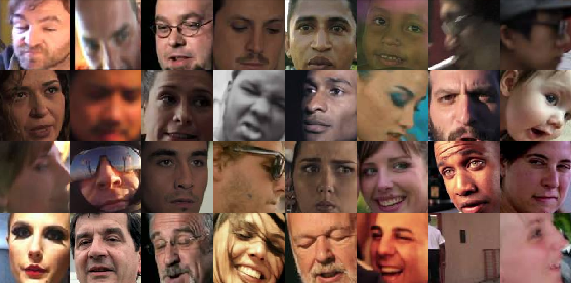
\includegraphics[width=0.98\linewidth]{img/random_sample_faces.png}
    \caption{A random selection of faces extracted from the dataset. In the bottom right corner we can see a false positive from extraction.}
    \label{fig:random_selection_faces}
\end{figure}

\section{Face similarity based on the deep features}

\todo{Since in this research area face features often represent face landmarks, in this chapter we will use term face encodings for the s high-dimensional descriptor of the face.}

First of all, we were interested if the features from pretrained network contain interesting information, that could help in the search for a specific face. We used ... \todo[inline]{Add dlib more information}. This network produces a feature vector of length 128 as face representation. The authors' state, that the recommended threshold for euclidean distance for two feature vectors to be accepted as one is 0.6.

We investigated the results based on the euclidean distance and we show a result for a given face to find the closest (i.e., most similar) faces in the dataset. The sample can be seen in the figure \ref{fig:closest_faces}.


\begin{figure}
    \centering
    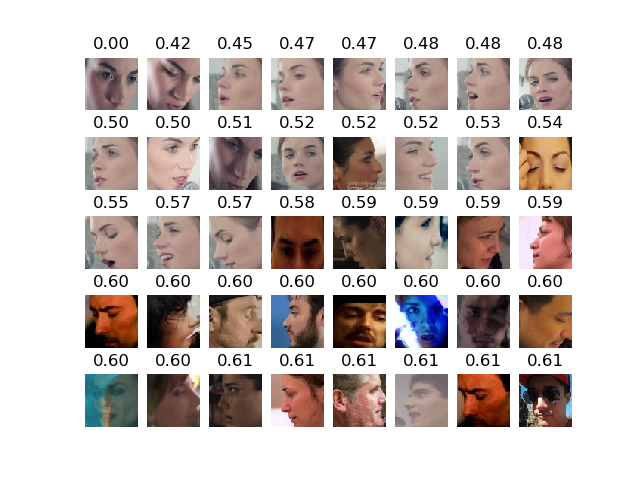
\includegraphics[width=\linewidth]{img/closest_faces_to_woman.png}
    \caption{Examples of the retrieved closest faces to the query face (top left) based on euclidean distance. Above images is the distance from the query.}
    \label{fig:closest_faces}
\end{figure}

\section{Case study}

The features we obtained in the previous step were created to perform well on the identification task. Therefore, we want to find out, if the space over the face features contains also information about the similarity between the faces. From the published results (\cite{}) we known that the model achieves state-of-art performance on the identification task.
\todo[inline]{Prohodit posledni dve vety?}

We conducted a study with 25 participants. We presented them a grid $10\times10$ of randomly selected faces from the dataset. 
Then we showed them 10 randomly selected target faces of different people. We asked the participant to select for each target face exactly three faces from the grid that looked the most similar. Out of 10 people in target images, one of them was a child and two others was presented in the grid.
%Then we asked them, to select exactly three faces, which are the most similar to the provided target face. Our test contained 10 randomly pre-selected faces of different people. Out of 10, one of them was a child, we estimate below 10 years old. Two of the other target faces were present in the grid.
One of them was extracted from the same image, i.e. the same angle of the face. The second of the target faces, which were shown in the grid, had two representants in the grid. One identical to the target face, the second one only with a minor change of the angle.

Twenty-four out of 25 respondents selected the face corresponding to the same target person in the first case. In the second case, two face views of the target person were available in the grid. 9 respondents selected both correctly and 11 respondents selected only one of them. We conclude, that only in 70.7\% of the cases users noticed the target person in the grid $10\times10$.

We further investigate the seven target faces, which were not present in the grid. For each of the faces from the grid we computed the Euclidean distance from the target face encoding \todo{kde se vzal, tu se vzal -- encoding!?} to them. We then reordered the faces from the grid based on this distance. The closest faces received had the lowest index over the sorted distances. We refer to the index of the face in the sorted set of faces as $rank$.

We were interested in the distribution of ranks given the faces selected by the users. This would show us, if there is any correlation between similarity in the feature space and the similarity percieved by the human respondents. From the survey responses we create a heatmap for each task. The size of the heatmap corresponds to the size of the face grid, i.e., $10\times10$. The element on the position $task, i, j$ of the heatmap corresponds to the number of times, the face at $i$-th row and in $j$-th column was selected in the given $task$. We use the heatmap and the ranking based on the distances in the feature space, to compute, how many closest faces from feature space were actually selected. We do the same for each rank. The normalized results over all possible ranks (from 0 to 99) are plotted in the figure \ref{fig:survey_distribution}. If the users perception was fully coherent with the ordering based on the distances in the feature space, the  
probability on the first three ranks (0,1,2) would be equal to 1. Even though we do not see such full coherence in the results, we can see a trend of decreasing probability of choosing a face by user with the increasing distance from the target face.

We also show a comparison to the performing only six tasks, excluding the one, where the target person was child. The used network for feature extraction as many other are not performing well on the children from the dataset. This is caused by fact that most of the available face datasets contain only adults. This causes the networks to often put children closer together, even though, they may be a different person. Encodings of two different children tend to be closer to each other compared to the encoding of the two adults (source: \href{https://face-recognition.readthedocs.io/en/latest/readme.html#caveats}{Face Recognition Caveats}). Therefore we can see a significant improvement over the lowest ranks, since selecting a child from the map resulted in smaller distances, compared to the adults.

As the last investigation from the case study we provide a graph displaying the expected value of the number of faces selected up to a given rank (figure \ref{fig:random_selection_faces}). On average, one of the three selected by the user, has rank less than 12. Base on the user study we showed that this feature space over face encodings provides us with some information about face similarities.

\begin{figure}
    \centering
    \begin{subfigure}[b]{0.48\textwidth}
     \centering
     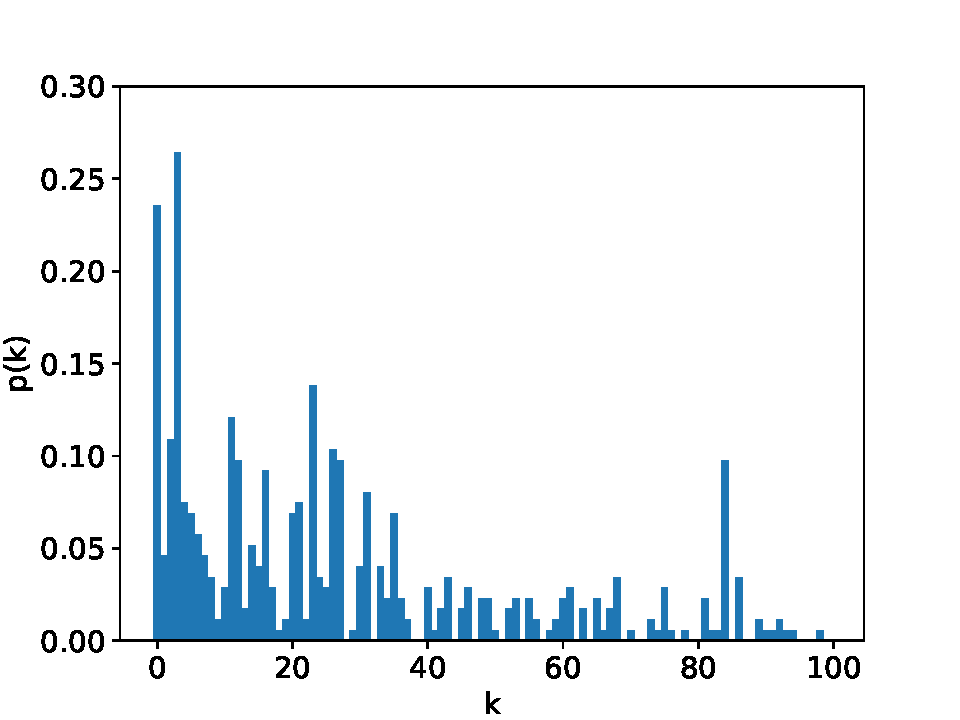
\includegraphics[width=\textwidth]{graphs/survey_distribution_without_the_easy.pdf}
     \caption{Performed on 7 task, which did not contain the target person in the grid}
     \label{fig:survey_all}
    \end{subfigure}
    \begin{subfigure}[b]{0.48\textwidth}
     \centering
     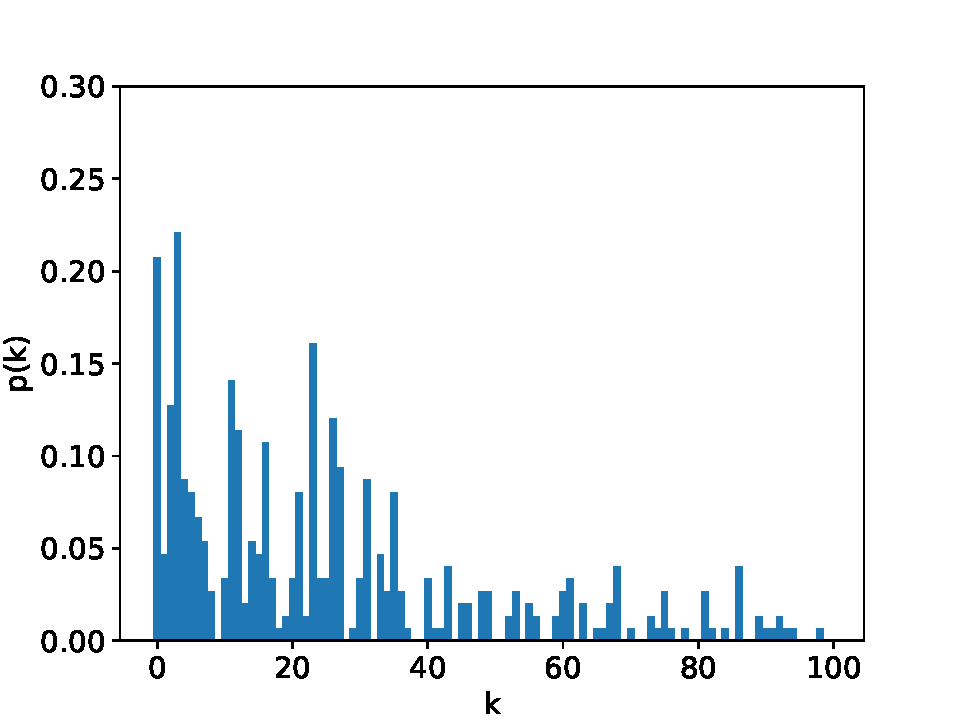
\includegraphics[width=\textwidth]{graphs/survey_distribution_childless.pdf}
     \caption{Performed on six tasks, extracting the task involving a child}
     \label{fig:suvery_childless}
    \end{subfigure}
    
    \caption{Collected statistic on how likely user selects $k$-th closest face to the target in the face grid. Ideally, if user was fully coherent with the distances in the features space, $p(k) = 1$ on [0, 2], since the user selected exactly 3 faces, and $p(k) = 0$ for all other $k$.}
    \label{fig:survey_distribution}
\end{figure}


\begin{figure}
    \centering
    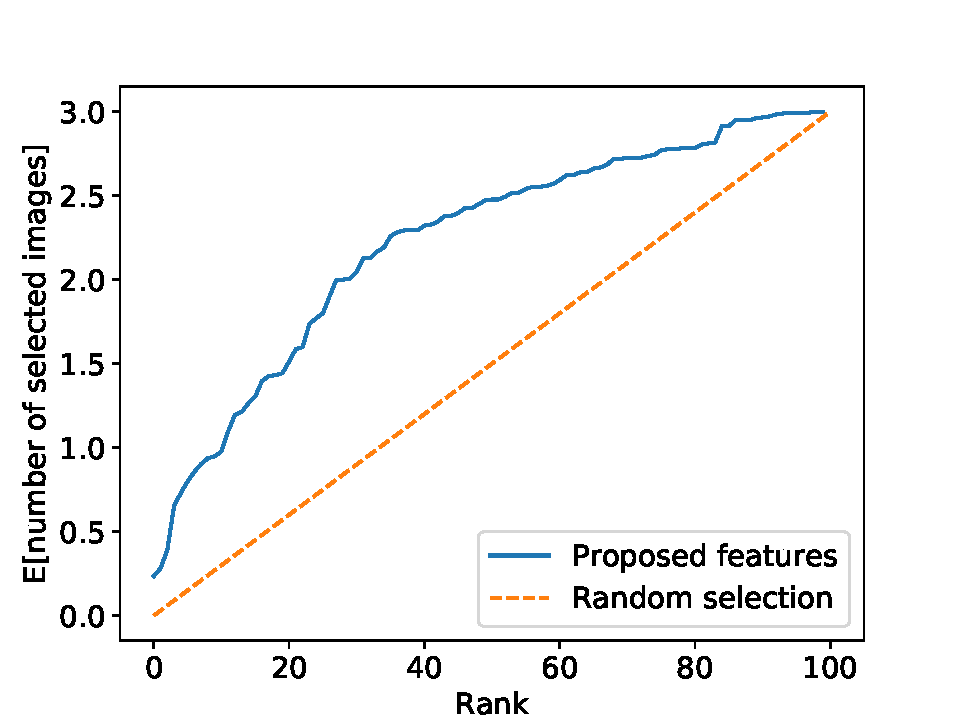
\includegraphics[width=0.8\linewidth]{graphs/survey_cumsum_without_the_easy.pdf}
    \caption{Expected value of the number of images selected up to a given rank.}
    \label{fig:my_label}
\end{figure}

\section{Building a traversal scheme}

In the previous sections, we obtained and encoded faces. We investigated the feature space based on the correspondence to the manual annotations in the case study. Here we propose a solution of organizing faces into a multilevel view. 

As we discussed in Related Work, a common solution for traversal system is a 2D grid. This usually allows users navigation queries, as left, right, top, bottom. We call a set of images, which is visible at a prticular step a \emph{display}. Display may contain from tens to hundreds images at once depending on multiple factor. One of the is a user's screen size, the size of the displayed image, etc.

Since most of the times, we want to display more data than small hundreds, it becomes incovieniet to preview dotaset only in a one layer. Therefore, we build a simple multilevel structure to ease the navigation, when moving by a greater distance.

\subsection{Tree-based structure}

Our goal is to organise a dataset of images $D$. Let us assume, that the dataset can be organized into a grid of size $N\times M$. We leave the choice of the specific dimensions to the user. We prefer more square setting, although, it is possible with any. In case, that the size of the dataset $|D|$ is almost a square of any number, we recommend adding a dummy image/s.

We organise (so far in non-specific way) the items from the dataset into a 2D grid. This is our base layer for the tree structure, we denote it as $L_0$. The overview of the structure is shown in the figure \ref{fig:tree_structure}. The layer has dimensions $L_{0, h}\times L_{0, w}$. Based on this layer, we create a next layer as only a subset of this layer. Firstly, we select a $k$, which represents the subset size factor. It means, that every $k^2$ image is selected as a representant to the next layer

The layer $L_{i+1}$ has $1/k$ of the size in both directions of the $L_i$. The item on the position $i, j$ in the $L_{i+1}$ is replicated from the layer $L_i$ on the coordinates $i * k, j*k$. We continue reducing the size of the layers, until the layer will fit as a display to user's screen.

In this structure we support six types of navigation: left, right, down, up, in, out. In and out represent operations between the layers and other directional commands navigate withing the layer. 

\todo[inline]{tu treba dopisat njeake spodna cela cast a celkovo opravit tu matiku}

\begin{figure}
    \centering
    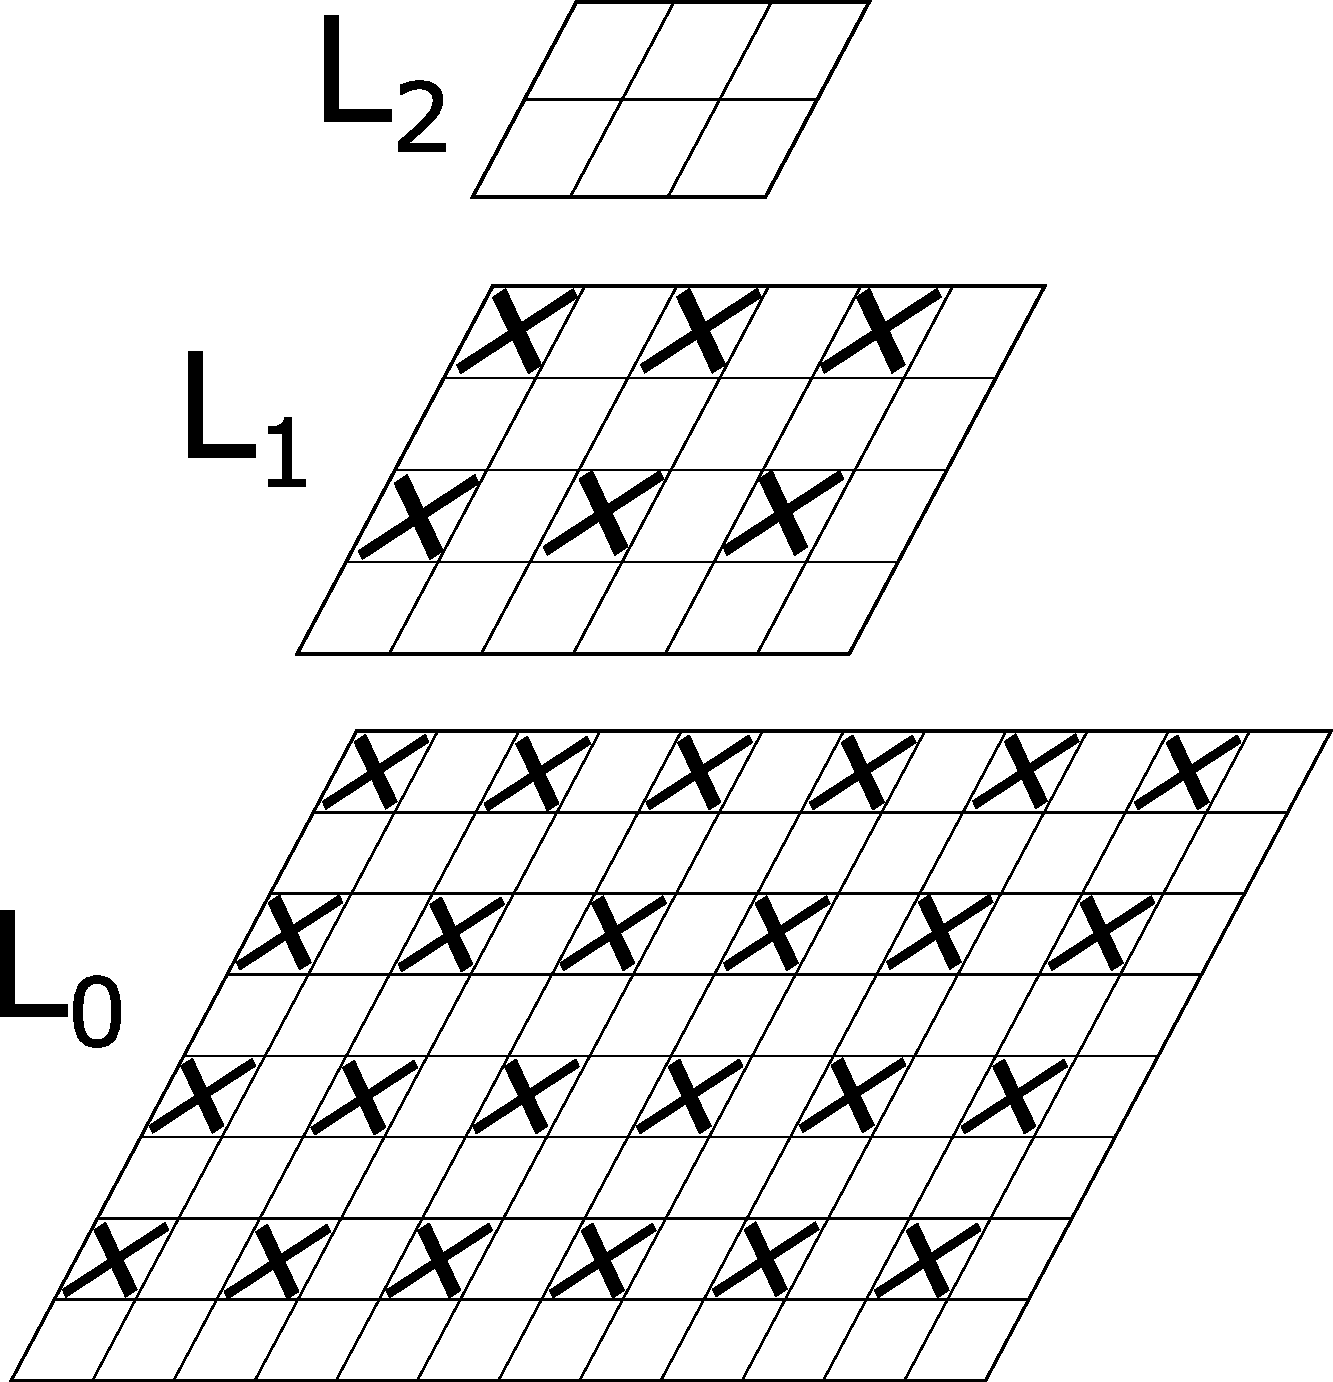
\includegraphics[width=0.3\linewidth]{img/tree-structure.pdf}
    \caption{A preview of the tree-based structure with $k = 2$ for previewing images. The marked items are selected for the layer above.}
    \label{fig:tree_structure}
\end{figure}

\section{Bottom Layer - Self organizing map}

In the bottom layer, we would like to make use of the face encodings. As we reviewd in Related Work, Self-organizing maps have the power to project high-dimensional data into 2D space. We train a self-organizing map on our dataset of face encodings. For our particular dataset, we train a network of size $50\times 50$. This offers us 2500 slots at the lowest layer, having more slots than faces in the dataset.

We trained the SOM for \todo{}. After the training, we assign to the each node of the SOM closest face in the feature space. This way we assign each of SOM nodes one representant. We investigated the representans, now projected into a grid, and we can observe, that after the training, faces corresponding to the same person are clustered together. In some parts of the map, there are duplicites. It means, that the same face is used as representant in multiple nodes. We evaluated how many of the faces are represented in the displayed set. \todo{} out of 2047 faces were matched to one of the SOM node.

\section{Evaluation}

In this section we present evaluation of the proposed, navigational system. The goal of this chapter was to propose exploration method over the dataset of faces. Therefore, we evaluate it by conducting an experiment including a user.

The task for the user is to find a target face in the dataset. As our baseline, we construct the grid of the faces, in random order. For searching in this grid a user can only scroll up and down through the dataset. We then test our traversal structure. The hypothesis we aim to prove is, that our solution decreases the average time needed to find the target face compared to the search in random dataset.

For our experiment we use the same 10 faces, as used for the case study. These were randomly selected from the dataset. For each of them we let the user search for the face in the dataset. Half of them is firstly searched in the "random view" and the other half is firstly searched via "traversal structure". We conduct the study among two subjects, providing us with 20 measurements.


\begin{figure}
    \centering
    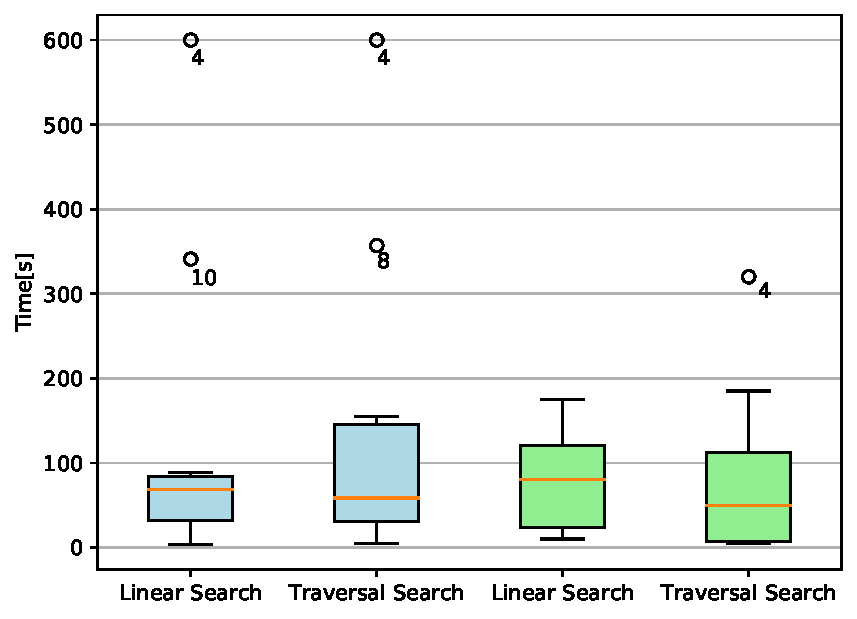
\includegraphics[width=0.7\linewidth]{graphs/face_search_time.pdf}
    \caption{Comparison of the time required to find a target image. Light blue belongs to the respondent A, light green to respondent B. The outliers are identified by the number of the query.}
    \label{fig:my_label}
\end{figure}